\documentclass{standalone}
\usepackage[svgnames]{xcolor}
\usepackage{tikz}
\usetikzlibrary{calc}
\usetikzlibrary{tikzmark}
\usetikzlibrary{arrows} % For nice arrow tips (Align-BDD)

\begin{document}
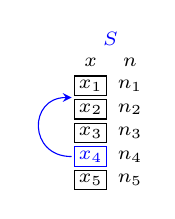
\begin{tikzpicture}[level distance=3mm,
  baseline=(current bounding box.center),
  sibling distance=5mm,
  font=\scriptsize,inner sep=1.5pt,
  labeln/.style={draw=black},
  weightn/.style={draw=none},
  edge from parent/.style={draw=none}]
  \node[draw=none]{\color{blue} $S$}
  child {node[draw=none] {$x$}
  child {node[labeln] (x1) {$x_1$}
    child {node[labeln] (x2) {$x_2$}
      child {node[labeln] {$x_3$}
        child {node[labeln, color=blue] (x4) {$x_4$}
          child {node[labeln] {$x_5$}}}}}}}
  child {node[draw=none] {$n$}
    child {node[weightn] {$n_1$}
      child {node[weightn] {$n_2$}
        child {node[weightn] {$n_3$}
          child {node[weightn] {$n_4$}
            child {node[weightn] {$n_5$}}}}}}};
  \draw (x4.west) edge[out=180, in=180, shorten >= 1pt, shorten <= 1pt, looseness=2.0, color=blue, -stealth] ($(x1.west)!.5!(x2.west)$);
\end{tikzpicture}%
\quad $\Rightarrow$\quad%
  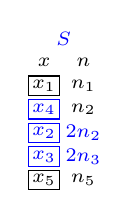
\begin{tikzpicture}[level distance=3mm,
    baseline=(current bounding box.center),
    sibling distance=5mm,
    font=\scriptsize,inner sep=1.5pt,
    labeln/.style={draw=black},
    weightn/.style={draw=none},
    edge from parent/.style={draw=none}]
    \node[draw=none]{\color{blue} $S$}
    child {node[draw=none] {$x$}
      child {node[labeln] {$x_1$}
        child {node[labeln, blue] {$x_4$}
          child {node[labeln, blue] {$x_2$}
            child {node[labeln, blue] {$x_3$}
              child {node[labeln] {$x_5$}}}}}}}
    child {node[draw=none] {$n$}
      child {node[weightn] {$n_1$}
        child {node[weightn] {$n_2$}
          child {node[weightn, blue] {$2n_2$}
            child {node[weightn, blue] {$2n_3$}
              child {node[weightn] {$n_5$}}}}}}};
  \end{tikzpicture}

  % \begin{tikzpicture}[%
  %   baseline=(current bounding box.center),
  %   level 1/.style={level distance=3mm},
  %   level 2/.style={level distance=4mm},
  %   sibling distance=8mm,
  %   font=\scriptsize,inner sep=2pt,
  %   labeln/.style={draw=black, minimum width=7mm},
  %   weightn/.style={draw=none},
  %   edge from parent/.style={draw=none}]
  %   \node[draw=none]{$S$}
  %   child {node[draw=none] {$x$}
  %     child {node[labeln] (i) {$x_i$}
  %       child {node[labeln] (ip1) {$x_{i+1}$}}}}
  %   child {node[draw=none] {$n$}
  %     child {node[weightn] {$n_i$}
  %       child {node[weightn] {$n_{i+1}$}}}};
  %   \draw (i.west) edge[out=180, in=180, shorten >= 1pt, shorten <= 1pt, looseness=2.0, color=NavyBlue, stealth-stealth] (ip1.west);
  % \end{tikzpicture}%
  % ~~$\Rightarrow$~~%
  % \begin{tikzpicture}[%
  %   baseline=(current bounding box.center),
  %   level 1/.style={level distance=3mm},
  %   level 2/.style={level distance=4mm},
  %   sibling distance=8mm,
  %   font=\scriptsize,inner sep=2pt,
  %   labeln/.style={draw=black, minimum width=7mm},
  %   weightn/.style={draw=none},
  %   edge from parent/.style={draw=none}]
  %   \node[draw=none]{$S^\prime$}
  %   child {node[draw=none] {$x$}
  %     child {node[labeln] {\color{NavyBlue} $x_{i+1}$}
  %       child {node[labeln] {\color{NavyBlue} $x_i$}}}}
  %   child {node[draw=none] {$n$}
  %     child {node[weightn] {$n_i$}
  %       child {node[weightn] {\color{NavyBlue} $2n_i$}}}};
  % \end{tikzpicture}%
\end{document}